% Options for packages loaded elsewhere
\PassOptionsToPackage{unicode}{hyperref}
\PassOptionsToPackage{hyphens}{url}
%
\documentclass[
]{book}
\usepackage{amsmath,amssymb}
\usepackage{lmodern}
\usepackage{ifxetex,ifluatex}
\ifnum 0\ifxetex 1\fi\ifluatex 1\fi=0 % if pdftex
  \usepackage[T1]{fontenc}
  \usepackage[utf8]{inputenc}
  \usepackage{textcomp} % provide euro and other symbols
\else % if luatex or xetex
  \usepackage{unicode-math}
  \defaultfontfeatures{Scale=MatchLowercase}
  \defaultfontfeatures[\rmfamily]{Ligatures=TeX,Scale=1}
\fi
% Use upquote if available, for straight quotes in verbatim environments
\IfFileExists{upquote.sty}{\usepackage{upquote}}{}
\IfFileExists{microtype.sty}{% use microtype if available
  \usepackage[]{microtype}
  \UseMicrotypeSet[protrusion]{basicmath} % disable protrusion for tt fonts
}{}
\makeatletter
\@ifundefined{KOMAClassName}{% if non-KOMA class
  \IfFileExists{parskip.sty}{%
    \usepackage{parskip}
  }{% else
    \setlength{\parindent}{0pt}
    \setlength{\parskip}{6pt plus 2pt minus 1pt}}
}{% if KOMA class
  \KOMAoptions{parskip=half}}
\makeatother
\usepackage{xcolor}
\IfFileExists{xurl.sty}{\usepackage{xurl}}{} % add URL line breaks if available
\IfFileExists{bookmark.sty}{\usepackage{bookmark}}{\usepackage{hyperref}}
\hypersetup{
  pdftitle={Brazil European Comparison of Air Traffic},
  pdfauthor={DECEA Performance Section, EUROCONTROL Performance Review Unit},
  hidelinks,
  pdfcreator={LaTeX via pandoc}}
\urlstyle{same} % disable monospaced font for URLs
\usepackage{color}
\usepackage{fancyvrb}
\newcommand{\VerbBar}{|}
\newcommand{\VERB}{\Verb[commandchars=\\\{\}]}
\DefineVerbatimEnvironment{Highlighting}{Verbatim}{commandchars=\\\{\}}
% Add ',fontsize=\small' for more characters per line
\usepackage{framed}
\definecolor{shadecolor}{RGB}{248,248,248}
\newenvironment{Shaded}{\begin{snugshade}}{\end{snugshade}}
\newcommand{\AlertTok}[1]{\textcolor[rgb]{0.94,0.16,0.16}{#1}}
\newcommand{\AnnotationTok}[1]{\textcolor[rgb]{0.56,0.35,0.01}{\textbf{\textit{#1}}}}
\newcommand{\AttributeTok}[1]{\textcolor[rgb]{0.77,0.63,0.00}{#1}}
\newcommand{\BaseNTok}[1]{\textcolor[rgb]{0.00,0.00,0.81}{#1}}
\newcommand{\BuiltInTok}[1]{#1}
\newcommand{\CharTok}[1]{\textcolor[rgb]{0.31,0.60,0.02}{#1}}
\newcommand{\CommentTok}[1]{\textcolor[rgb]{0.56,0.35,0.01}{\textit{#1}}}
\newcommand{\CommentVarTok}[1]{\textcolor[rgb]{0.56,0.35,0.01}{\textbf{\textit{#1}}}}
\newcommand{\ConstantTok}[1]{\textcolor[rgb]{0.00,0.00,0.00}{#1}}
\newcommand{\ControlFlowTok}[1]{\textcolor[rgb]{0.13,0.29,0.53}{\textbf{#1}}}
\newcommand{\DataTypeTok}[1]{\textcolor[rgb]{0.13,0.29,0.53}{#1}}
\newcommand{\DecValTok}[1]{\textcolor[rgb]{0.00,0.00,0.81}{#1}}
\newcommand{\DocumentationTok}[1]{\textcolor[rgb]{0.56,0.35,0.01}{\textbf{\textit{#1}}}}
\newcommand{\ErrorTok}[1]{\textcolor[rgb]{0.64,0.00,0.00}{\textbf{#1}}}
\newcommand{\ExtensionTok}[1]{#1}
\newcommand{\FloatTok}[1]{\textcolor[rgb]{0.00,0.00,0.81}{#1}}
\newcommand{\FunctionTok}[1]{\textcolor[rgb]{0.00,0.00,0.00}{#1}}
\newcommand{\ImportTok}[1]{#1}
\newcommand{\InformationTok}[1]{\textcolor[rgb]{0.56,0.35,0.01}{\textbf{\textit{#1}}}}
\newcommand{\KeywordTok}[1]{\textcolor[rgb]{0.13,0.29,0.53}{\textbf{#1}}}
\newcommand{\NormalTok}[1]{#1}
\newcommand{\OperatorTok}[1]{\textcolor[rgb]{0.81,0.36,0.00}{\textbf{#1}}}
\newcommand{\OtherTok}[1]{\textcolor[rgb]{0.56,0.35,0.01}{#1}}
\newcommand{\PreprocessorTok}[1]{\textcolor[rgb]{0.56,0.35,0.01}{\textit{#1}}}
\newcommand{\RegionMarkerTok}[1]{#1}
\newcommand{\SpecialCharTok}[1]{\textcolor[rgb]{0.00,0.00,0.00}{#1}}
\newcommand{\SpecialStringTok}[1]{\textcolor[rgb]{0.31,0.60,0.02}{#1}}
\newcommand{\StringTok}[1]{\textcolor[rgb]{0.31,0.60,0.02}{#1}}
\newcommand{\VariableTok}[1]{\textcolor[rgb]{0.00,0.00,0.00}{#1}}
\newcommand{\VerbatimStringTok}[1]{\textcolor[rgb]{0.31,0.60,0.02}{#1}}
\newcommand{\WarningTok}[1]{\textcolor[rgb]{0.56,0.35,0.01}{\textbf{\textit{#1}}}}
\usepackage{longtable,booktabs,array}
\usepackage{calc} % for calculating minipage widths
% Correct order of tables after \paragraph or \subparagraph
\usepackage{etoolbox}
\makeatletter
\patchcmd\longtable{\par}{\if@noskipsec\mbox{}\fi\par}{}{}
\makeatother
% Allow footnotes in longtable head/foot
\IfFileExists{footnotehyper.sty}{\usepackage{footnotehyper}}{\usepackage{footnote}}
\makesavenoteenv{longtable}
\usepackage{graphicx}
\makeatletter
\def\maxwidth{\ifdim\Gin@nat@width>\linewidth\linewidth\else\Gin@nat@width\fi}
\def\maxheight{\ifdim\Gin@nat@height>\textheight\textheight\else\Gin@nat@height\fi}
\makeatother
% Scale images if necessary, so that they will not overflow the page
% margins by default, and it is still possible to overwrite the defaults
% using explicit options in \includegraphics[width, height, ...]{}
\setkeys{Gin}{width=\maxwidth,height=\maxheight,keepaspectratio}
% Set default figure placement to htbp
\makeatletter
\def\fps@figure{htbp}
\makeatother
\setlength{\emergencystretch}{3em} % prevent overfull lines
\providecommand{\tightlist}{%
  \setlength{\itemsep}{0pt}\setlength{\parskip}{0pt}}
\setcounter{secnumdepth}{5}
\usepackage{booktabs}
\usepackage{amsthm}
\makeatletter
\def\thm@space@setup{%
  \thm@preskip=8pt plus 2pt minus 4pt
  \thm@postskip=\thm@preskip
}
\makeatother
\ifluatex
  \usepackage{selnolig}  % disable illegal ligatures
\fi
\usepackage[]{natbib}
\bibliographystyle{apalike}

\title{Brazil European Comparison of Air Traffic}
\author{DECEA Performance Section, EUROCONTROL Performance Review Unit}
\date{2021-04-26}

\begin{document}
\maketitle

{
\setcounter{tocdepth}{1}
\tableofcontents
}
\hypertarget{prerequisites}{%
\chapter{Prerequisites}\label{prerequisites}}

This project does something.

\begin{Shaded}
\begin{Highlighting}[]
\CommentTok{\# load BRA data}
\NormalTok{bra }\OtherTok{\textless{}{-}} \FunctionTok{c}\NormalTok{(}\DecValTok{2021}\NormalTok{)}
\NormalTok{eur }\OtherTok{\textless{}{-}} \FunctionTok{c}\NormalTok{(}\DecValTok{2021}\NormalTok{)}

\NormalTok{x }\OtherTok{\textless{}{-}}\NormalTok{ bra }\SpecialCharTok{+}\NormalTok{ eur}
\end{Highlighting}
\end{Shaded}

This is the sexy combination 4042.

\hypertarget{intro}{%
\chapter{Introduction}\label{intro}}

\hypertarget{introduction}{%
\chapter{Introduction}\label{introduction}}

The present briefing aims to provide a comparison of the COVID-19 impacts on aviation in different parts of the world. The regions covered herein are Europe, Brazil, Thailand, and Singapore.

\hypertarget{scope}{%
\chapter{Scope}\label{scope}}

The following airports are covered by this briefing:

\hypertarget{europe-airports}{%
\section{Europe airports}\label{europe-airports}}

EDDF, EDDM, EGLL, EHAM, LEMD, LFPG, LIRF, and LSZH

\hypertarget{brazil-airports}{%
\section{Brazil airports}\label{brazil-airports}}

SBBR, SBCF, SBCT, SBFL, SBGL, SBGR, SBKP, SBPA, SBRF, SBRJ, SBSP, and SBSV

\hypertarget{thailand-airports}{%
\section{Thailand airports}\label{thailand-airports}}

VTBD, VTBS, VTCC, and VTSP

\hypertarget{singapore-airports}{%
\section{Singapore airports}\label{singapore-airports}}

WSSS

\hypertarget{overview-comparison}{%
\chapter{Overview comparison}\label{overview-comparison}}

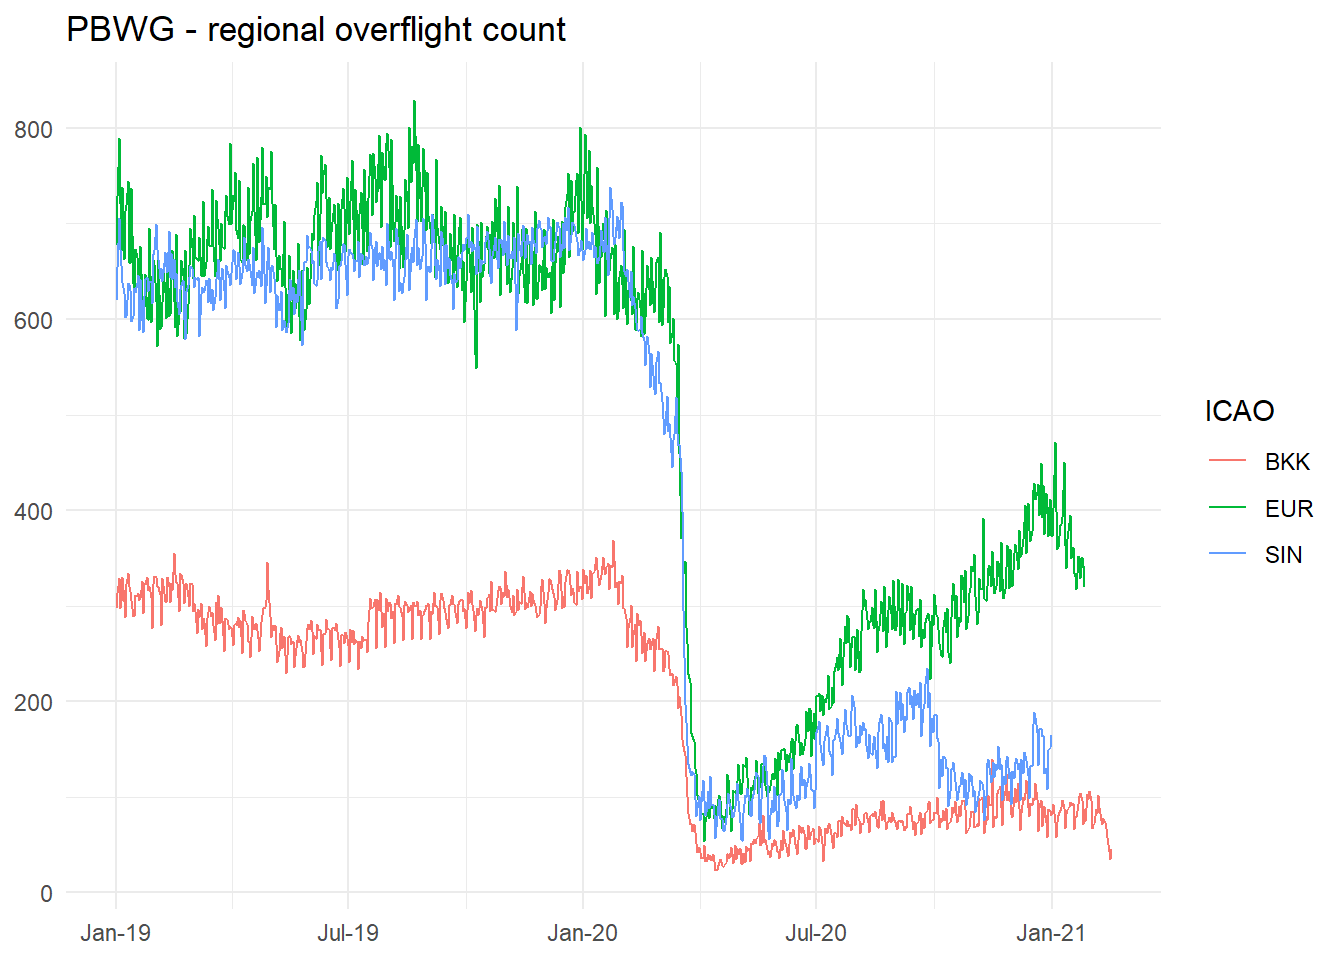
\includegraphics{bookdown-demo_files/figure-latex/unnamed-chunk-5-1.pdf}

\hypertarget{overflights}{%
\section{Overflights}\label{overflights}}

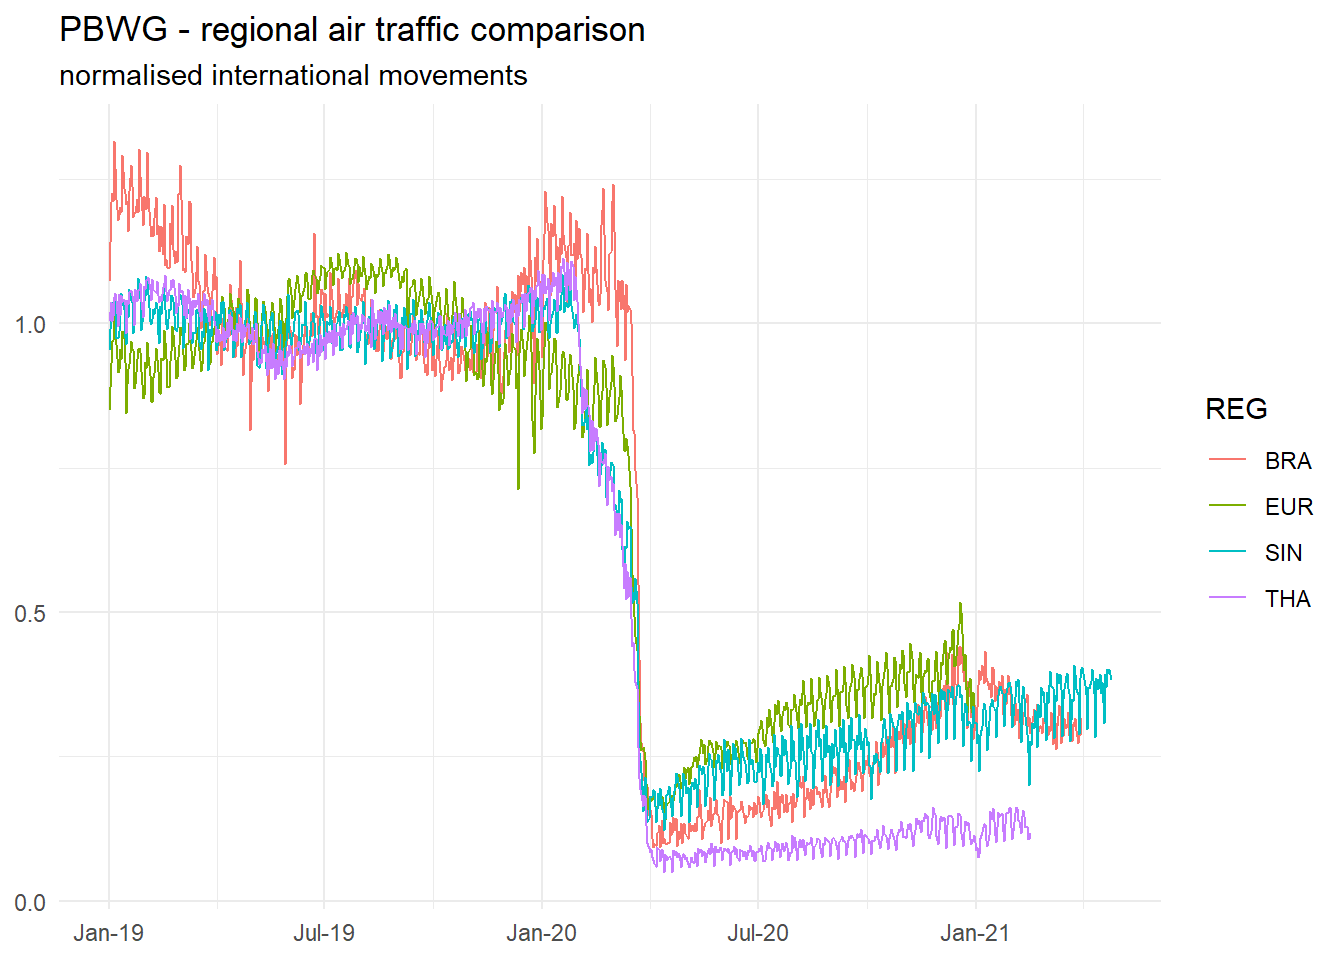
\includegraphics{bookdown-demo_files/figure-latex/unnamed-chunk-6-1.pdf}

\hypertarget{international-traffic}{%
\section{International traffic}\label{international-traffic}}

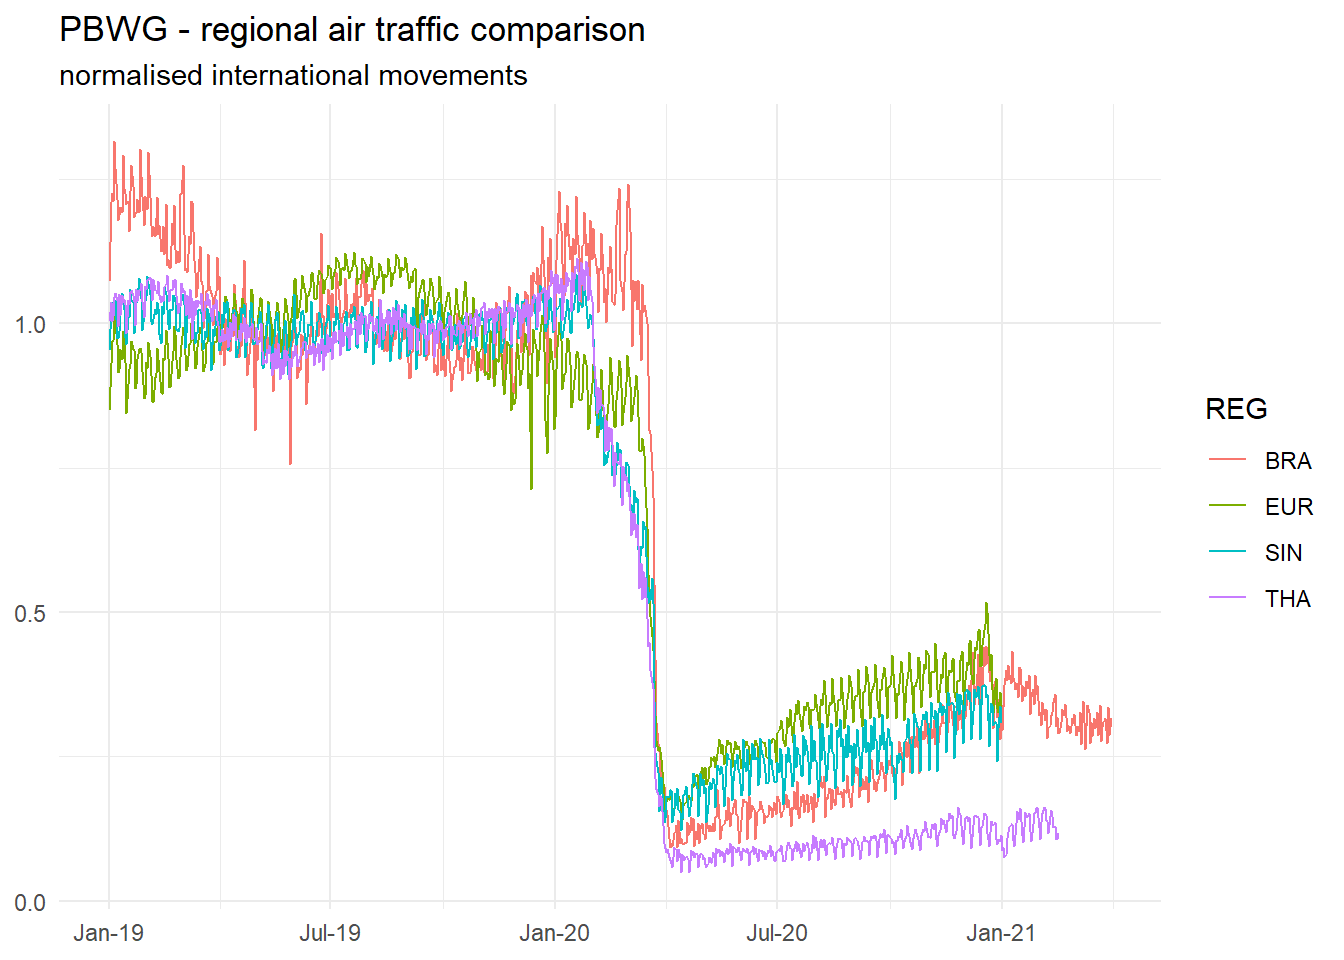
\includegraphics{bookdown-demo_files/figure-latex/unnamed-chunk-7-1.pdf}

\hypertarget{region-level-breakdown}{%
\chapter{Region level breakdown}\label{region-level-breakdown}}

\hypertarget{brazil}{%
\section{Brazil}\label{brazil}}

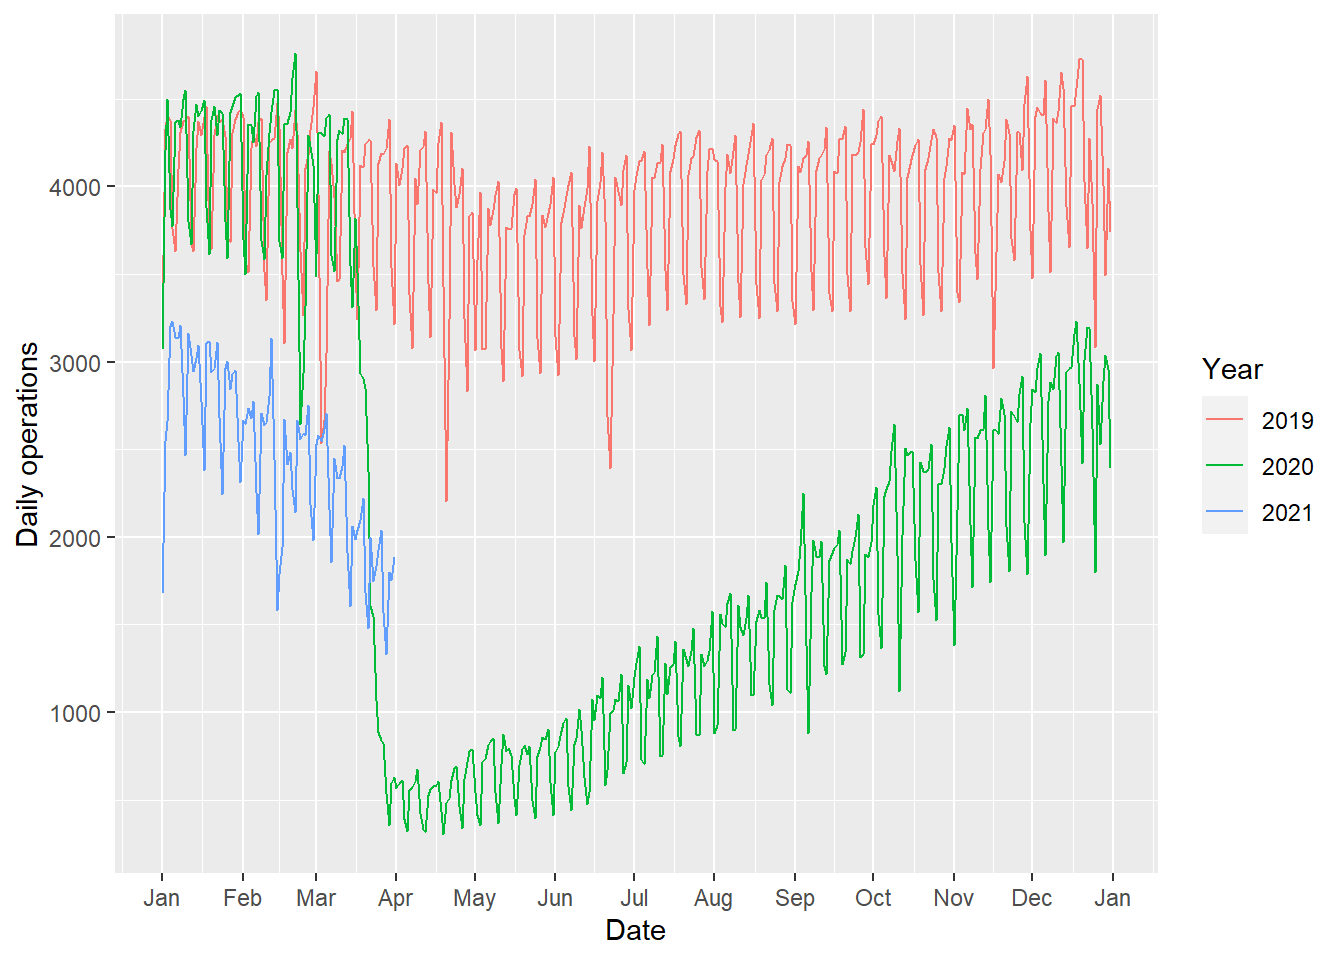
\includegraphics{bookdown-demo_files/figure-latex/unnamed-chunk-8-1.pdf}

\hypertarget{europe}{%
\section{Europe}\label{europe}}

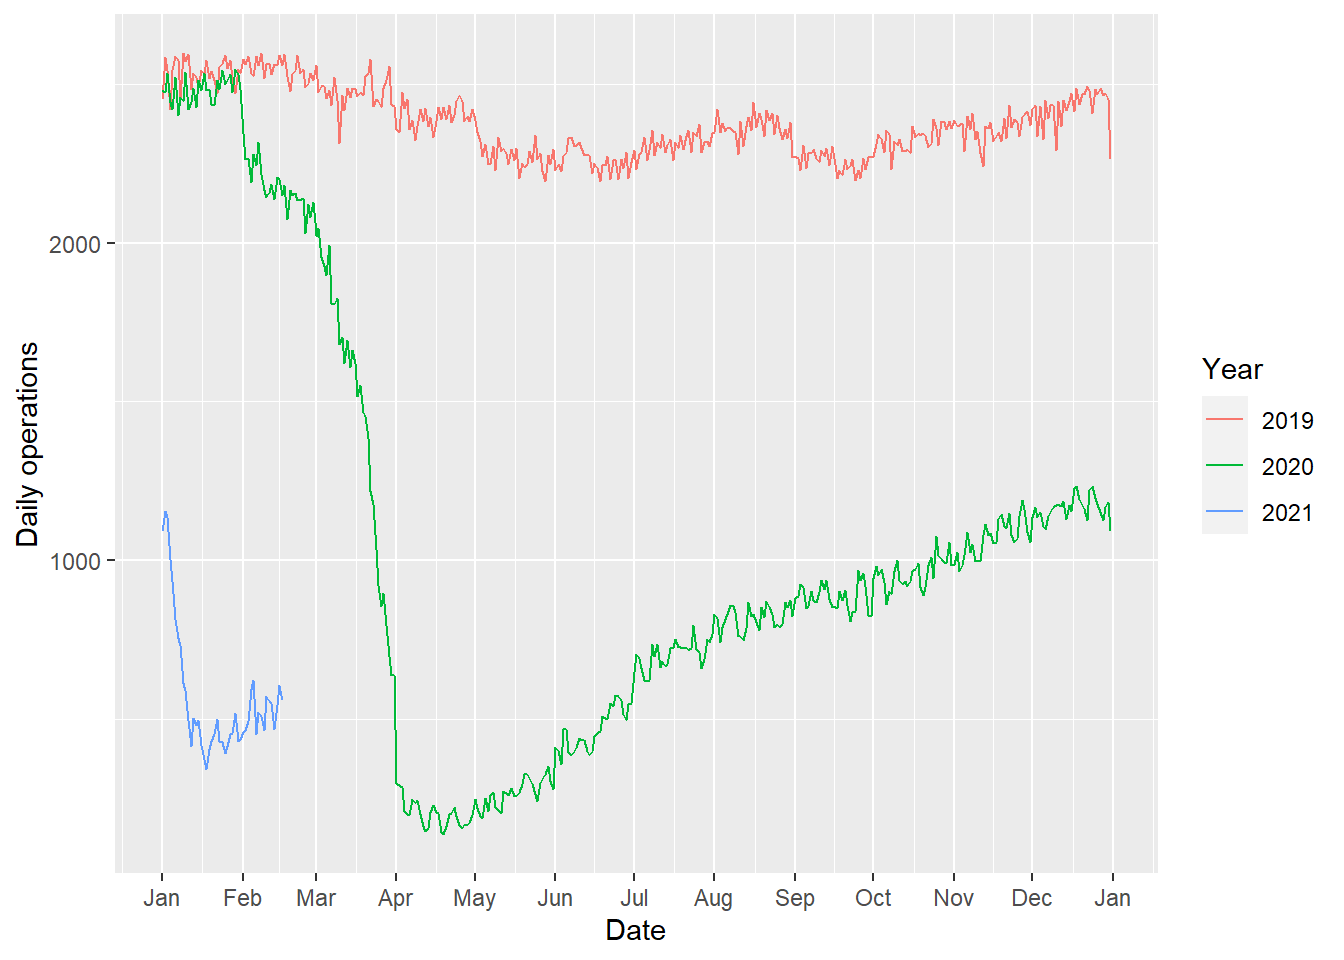
\includegraphics{bookdown-demo_files/figure-latex/unnamed-chunk-9-1.pdf}

\hypertarget{thailand}{%
\section{Thailand}\label{thailand}}

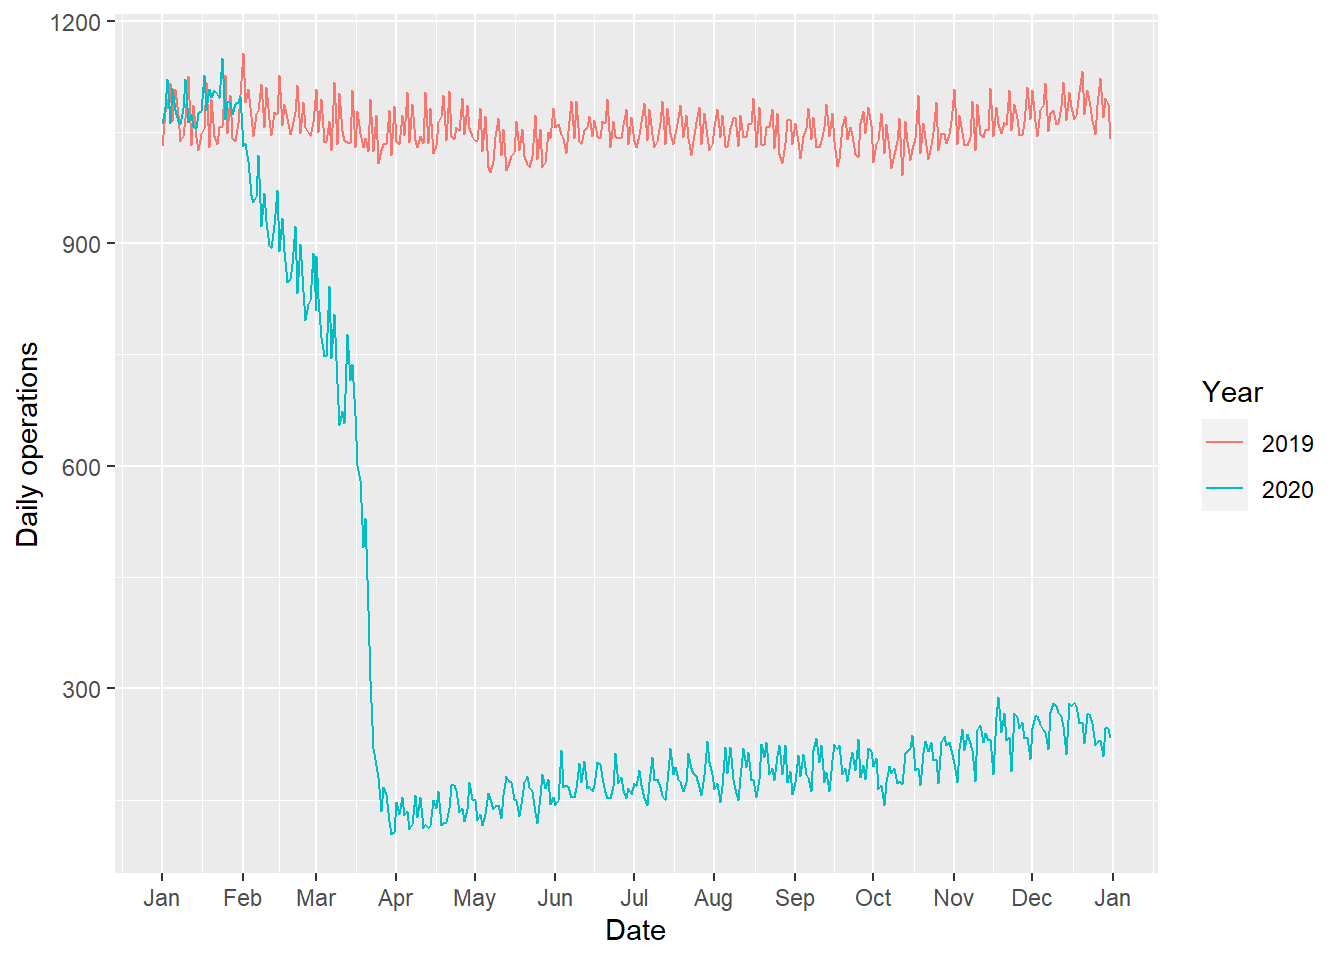
\includegraphics{bookdown-demo_files/figure-latex/unnamed-chunk-10-1.pdf}

\hypertarget{singapore}{%
\section{Singapore}\label{singapore}}

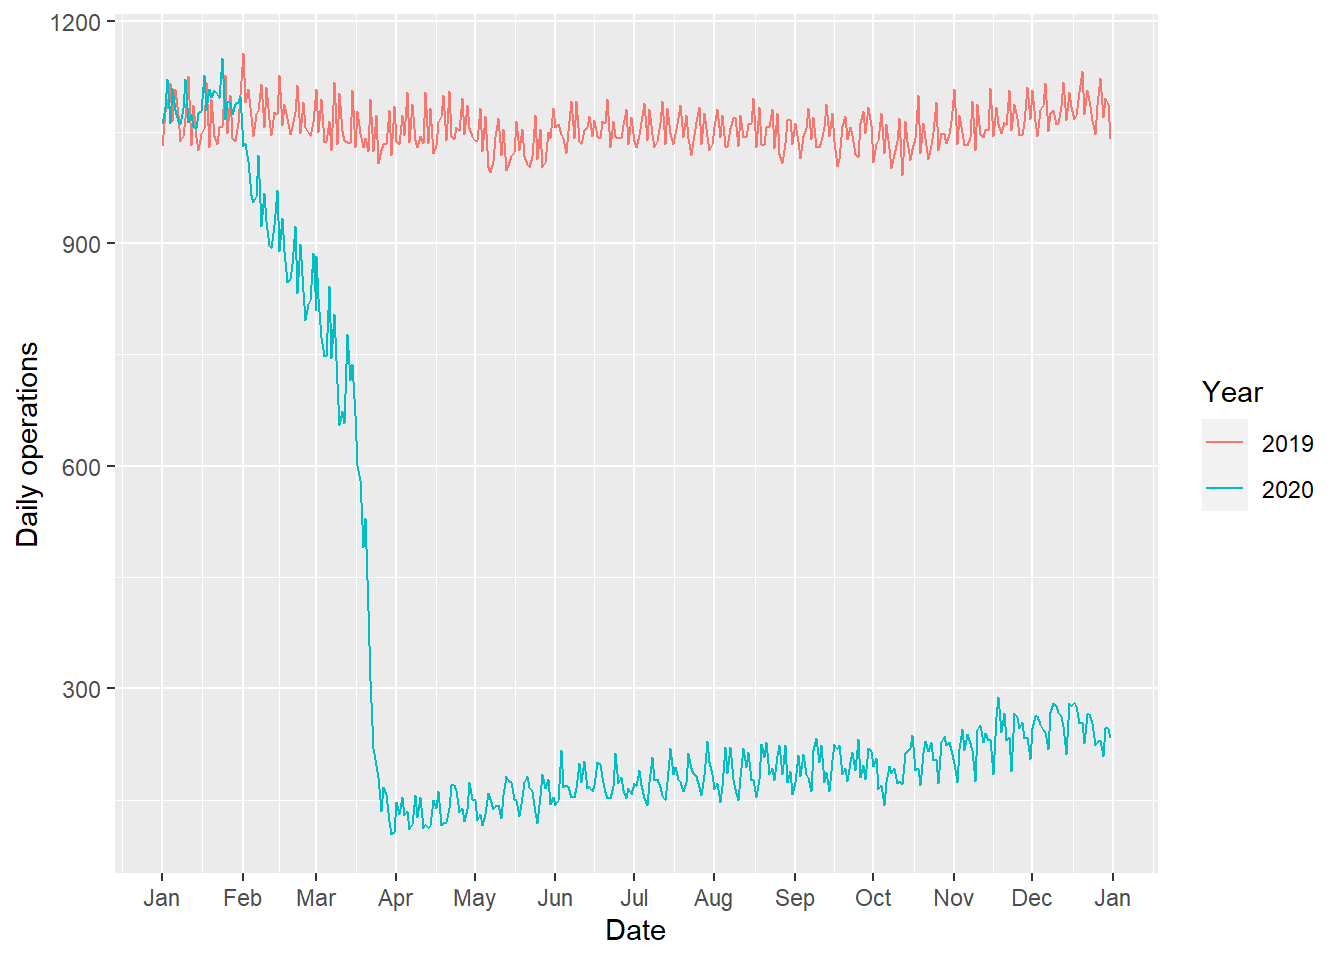
\includegraphics{bookdown-demo_files/figure-latex/unnamed-chunk-11-1.pdf}

\hypertarget{airport-level-breakdown}{%
\chapter{Airport level breakdown}\label{airport-level-breakdown}}

Except for Singapore, which has only one airport in the study, it is possible to look the different effects on individual airports within each region.

\hypertarget{brazil-airports-1}{%
\section{Brazil airports}\label{brazil-airports-1}}

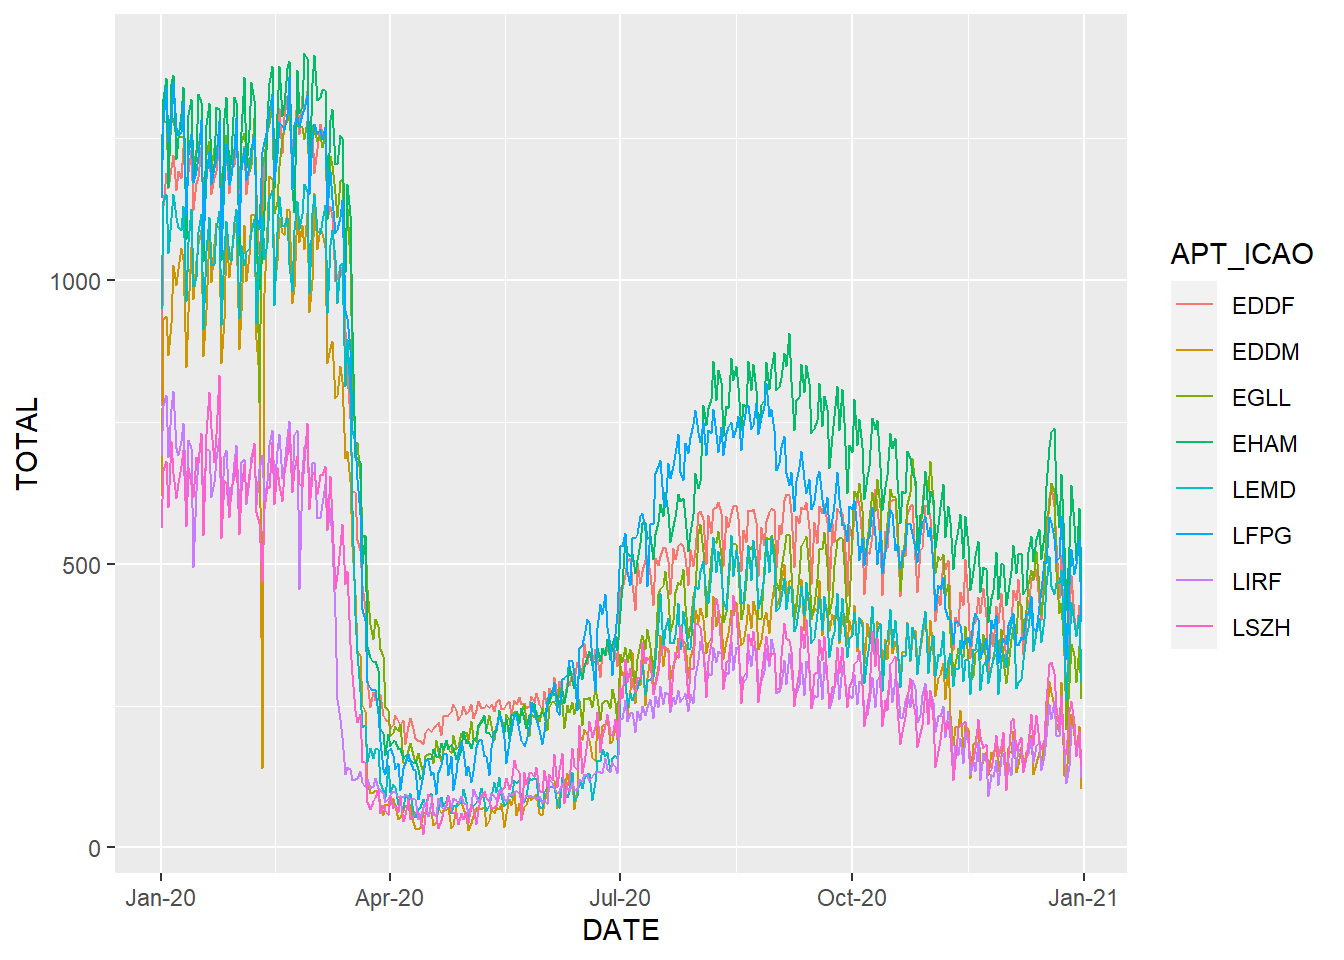
\includegraphics{bookdown-demo_files/figure-latex/unnamed-chunk-12-1.pdf} 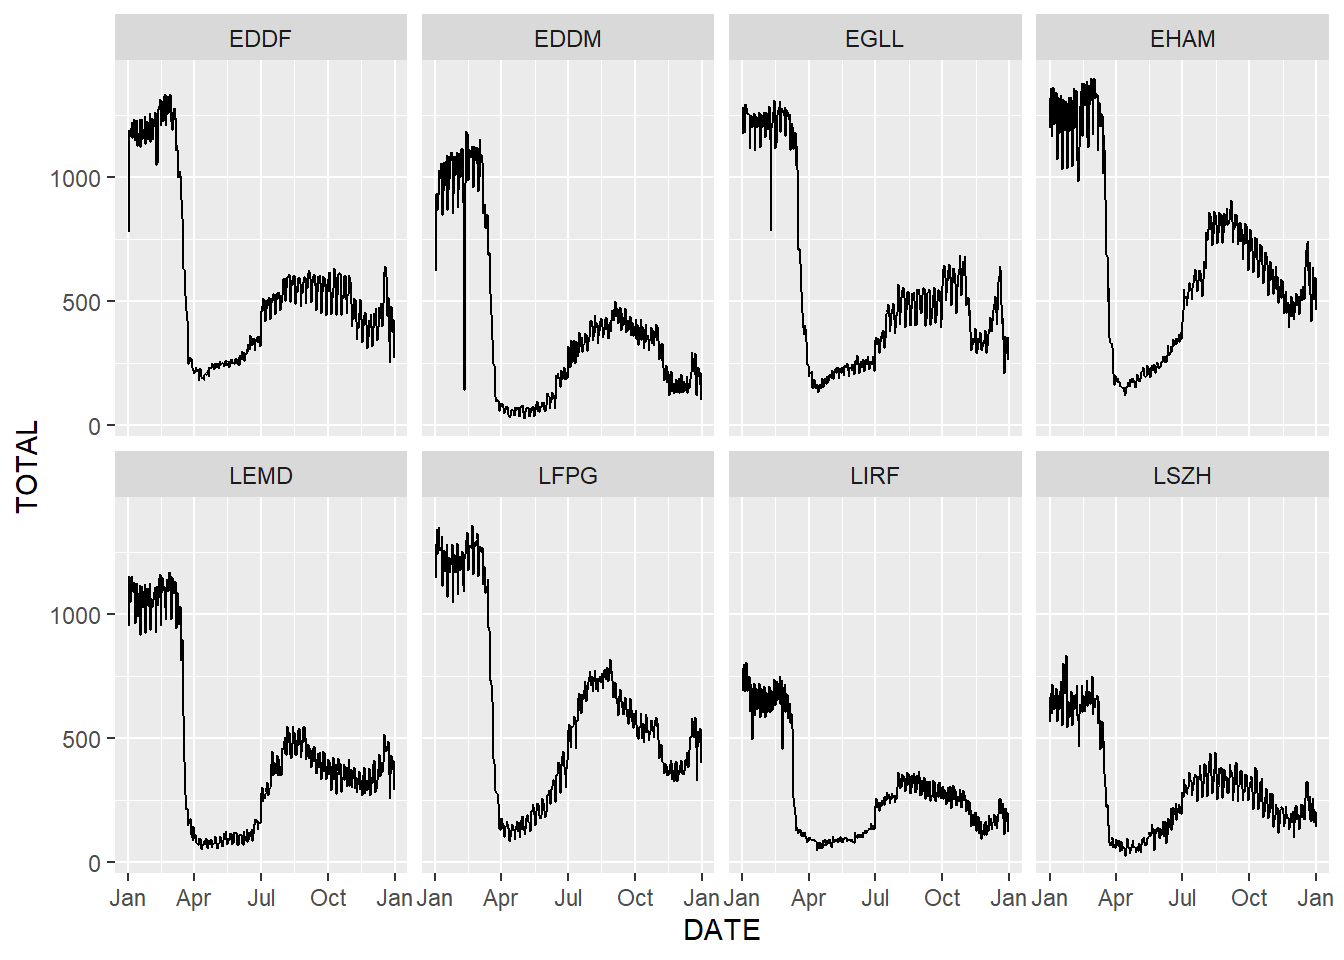
\includegraphics{bookdown-demo_files/figure-latex/unnamed-chunk-12-2.pdf}

\hypertarget{europe-airports-1}{%
\section{Europe airports}\label{europe-airports-1}}

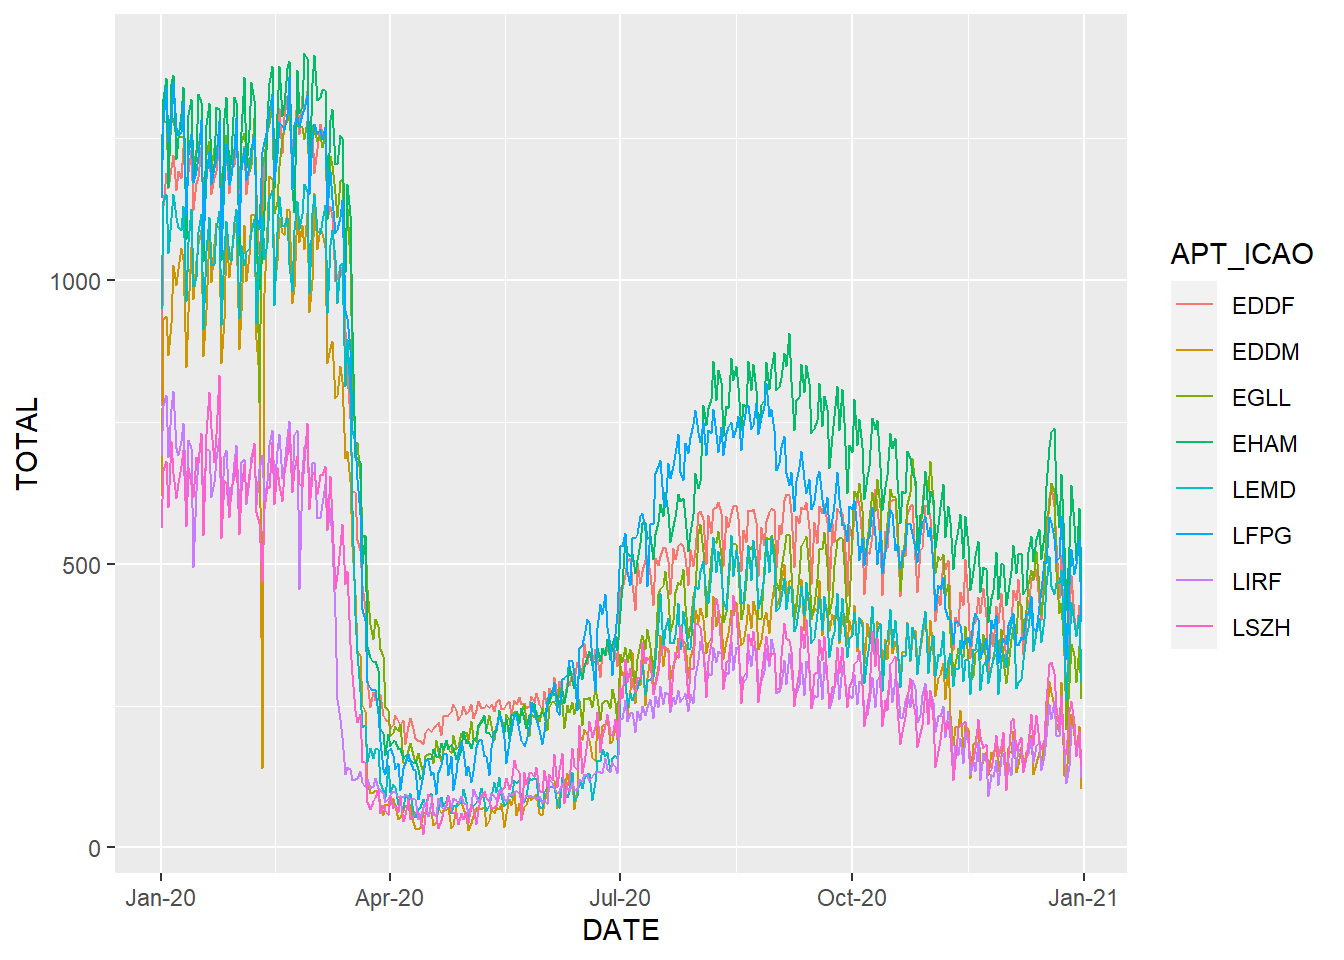
\includegraphics{bookdown-demo_files/figure-latex/unnamed-chunk-13-1.pdf} 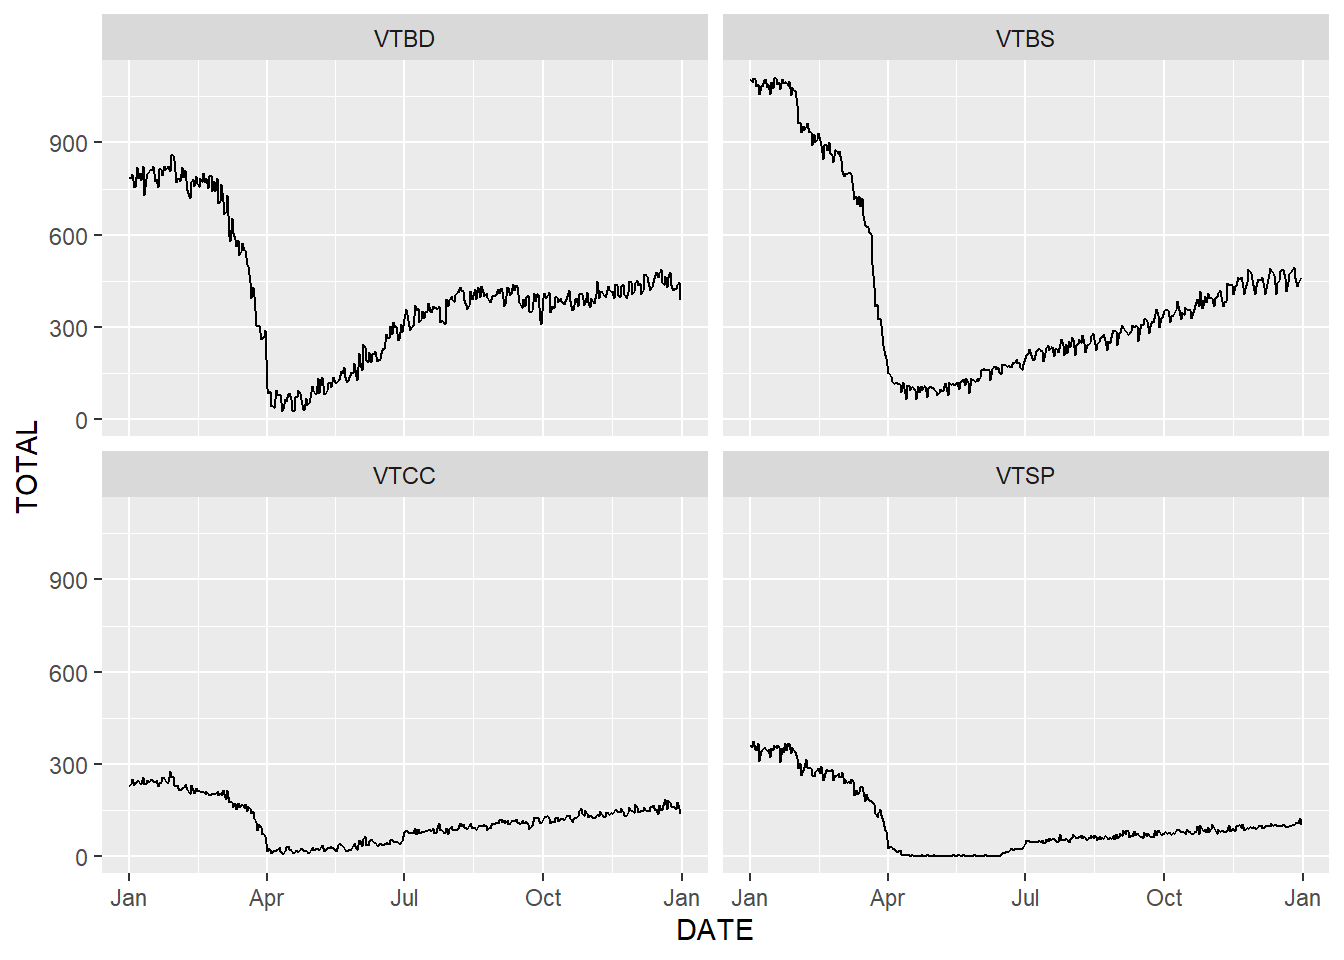
\includegraphics{bookdown-demo_files/figure-latex/unnamed-chunk-13-2.pdf}

\hypertarget{thailand-airports-1}{%
\section{Thailand airports}\label{thailand-airports-1}}

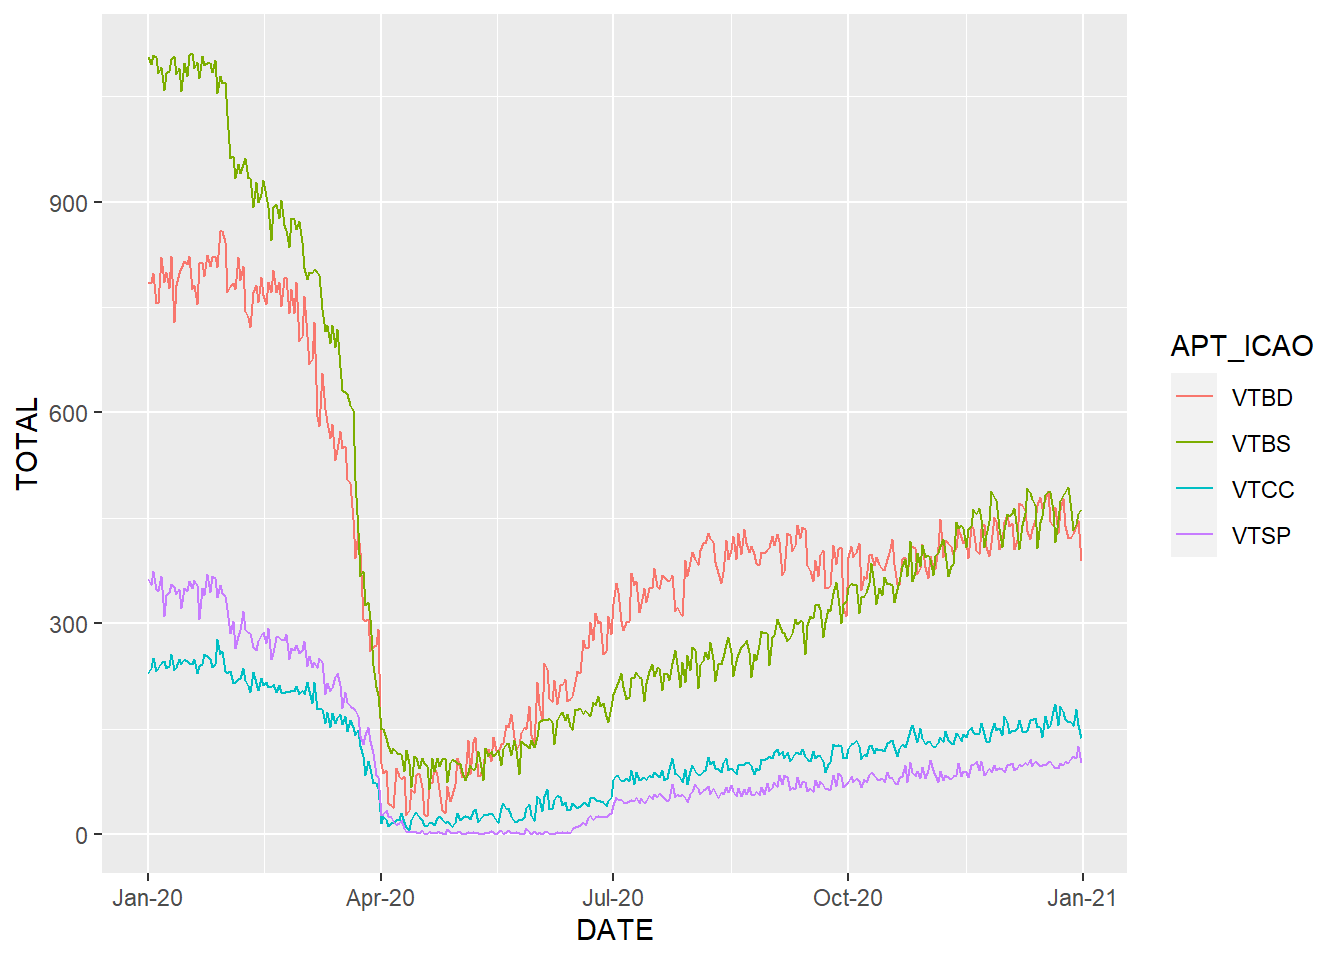
\includegraphics{bookdown-demo_files/figure-latex/unnamed-chunk-14-1.pdf} 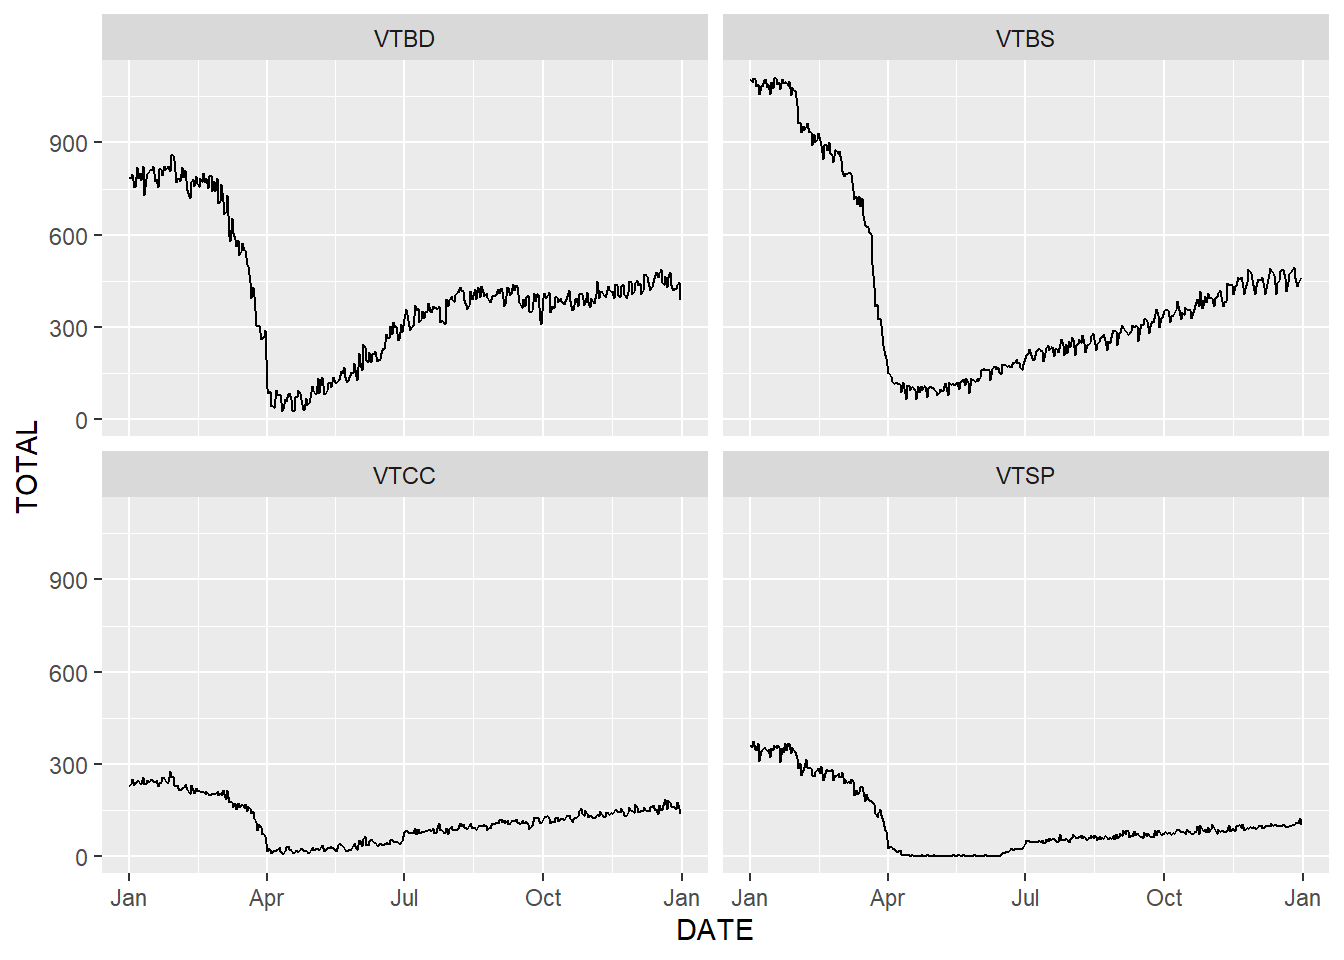
\includegraphics{bookdown-demo_files/figure-latex/unnamed-chunk-14-2.pdf}

\hypertarget{top-city-pairs}{%
\chapter{Top city pairs}\label{top-city-pairs}}

\hypertarget{brazil-routes}{%
\section{Brazil routes}\label{brazil-routes}}

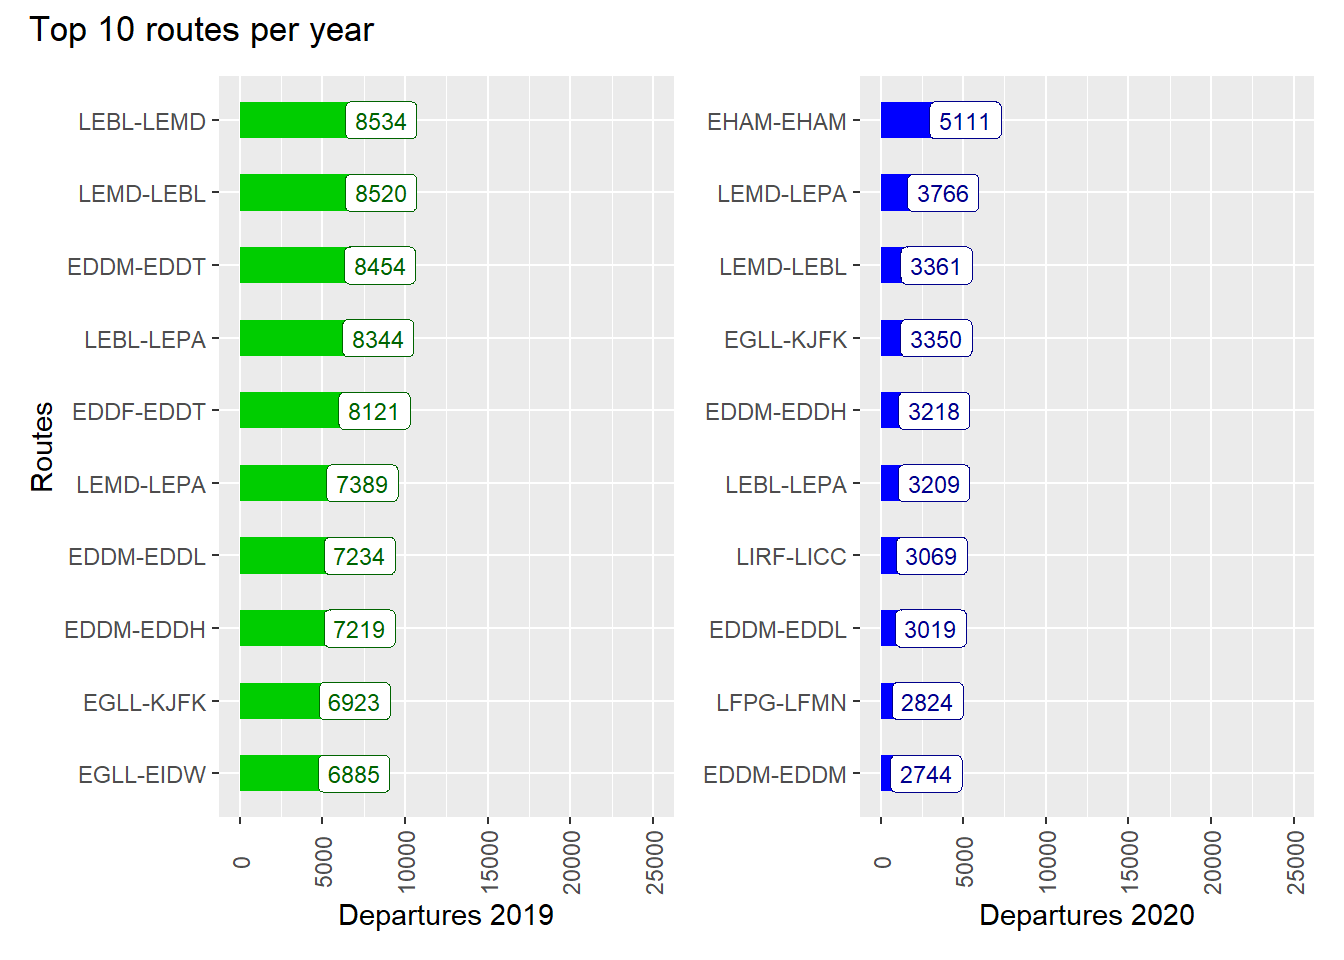
\includegraphics{bookdown-demo_files/figure-latex/unnamed-chunk-16-1.pdf}

\hypertarget{europe-routes}{%
\section{Europe routes}\label{europe-routes}}

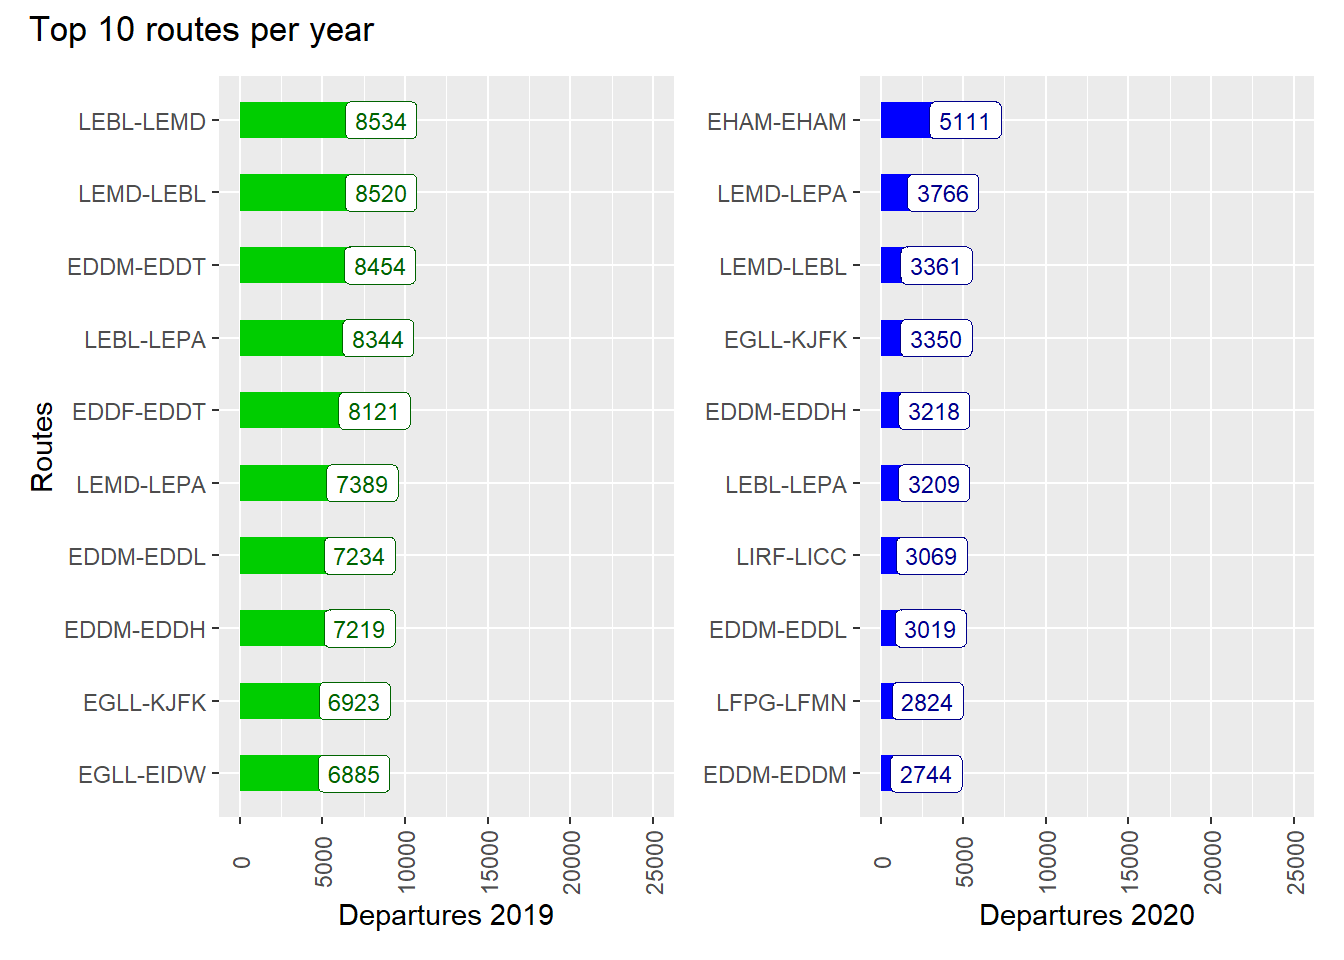
\includegraphics{bookdown-demo_files/figure-latex/unnamed-chunk-17-1.pdf}

  \bibliography{book.bib,packages.bib}

\end{document}
